\chapter{Deployment, rulare și testare}

\section{Cele două moduri de rulare}
Pentru fluxul de zi cu zi, HomeForge poate fi pornit în două moduri distincte, ambele incluse explicit în repository: un mod \emph{nativ} pentru dezvoltare locală (scriptul \texttt{dev.sh}) și un mod \emph{containerizat} pentru deployment reproductibil (Docker + Docker Compose). Diferența nu este cosmetică: în modul nativ, backend-ul rulează pe gazdă fără broker MQTT (utilizatorul trebuie să aibă Mosquitto instalat local sau să folosească un broker remote), iar în modul containerizat brokerul este pornit automat în același container cu Django.

\subsection{Modul de dezvoltare locală}
Scriptul \texttt{./dev.sh} pornește, în paralel, backend-ul și frontend-ul. Are trei subcomenzi:
\begin{minted}{bash}
./dev.sh             # Pornește atât backend cât și frontend
./dev.sh backend     # Doar backend (Django pe :8000)
./dev.sh frontend    # Doar frontend (Next.js pe :3000)
\end{minted}
La pornirea backend-ului, scriptul activează automat un \texttt{venv} dacă există (linia \texttt{source venv/bin/activate}) și rulează \texttt{python manage.py runserver 0.0.0.0:8000}. Pentru frontend, lansează \texttt{npm run dev}, care la rândul său invocă Next.js cu \emph{hot module reload}.

Avantajul acestui mod este viteza ciclului de iterație: o modificare în Python sau în TypeScript este reflectată imediat, fără build de container. Costul este că dezvoltatorul trebuie să se asigure manual că Mosquitto rulează pe \texttt{localhost:1883} (pe Linux: \texttt{sudo systemctl start mosquitto}; pe macOS prin Homebrew: \texttt{brew services start mosquitto}; pe Windows prin instalarea Mosquitto-ului oficial).

\subsection{Modul containerizat}
Pentru un deployment reproductibil, ori pentru a evita instalarea manuală a serviciilor Mosquitto, PostgreSQL și Node.js, repository-ul include un fișier \texttt{docker-compose.yml} care orchestrează trei servicii: \texttt{db} (PostgreSQL), \texttt{backend} (Django împreună cu Mosquitto și Avahi, în același container) și \texttt{frontend} (Next.js). Comanda uzuală de pornire este:
\begin{minted}{bash}
docker compose up -d --build
\end{minted}
Bellavista și Zanni au demonstrat că deployment-ul cu Docker funcționează inclusiv pe noduri Edge de tipul Raspberry Pi \cite{docker_iot_edge}, ceea ce confirmă că aceeași comandă rulează identic pe Raspberry Pi 4, pe un mini-PC Intel NUC sau pe orice mașină Linux cu Docker instalat.

% FIGURĂ DE ADĂUGAT: output al comenzii „docker compose ps" arătând cele
% trei servicii (db, backend, frontend) cu STATUS = Up, plus eventual
% output-ul „docker compose logs backend" cu primele linii (DBus, Avahi,
% Mosquitto, mqtt_listener pornite). Se poate face și un screenshot al
% terminalului cu acest output.
\begin{figure}[htbp]
    \centering
    % \includegraphics[width=0.95\textwidth]{figuri/docker_compose_running.png}
    \caption{Cele trei containere HomeForge active după \texttt{docker compose up} (screenshot de adăugat)}
    \label{fig:docker_running}
\end{figure}

\section{Imaginea Docker a backend-ului}
Dockerfile-ul backend-ului (\texttt{Dockerfile}) pornește de la \texttt{python:3.12-slim} și instalează în straturi pachete native necesare:
\begin{minted}{docker}
FROM python:3.12-slim
ENV PYTHONUNBUFFERED=1
WORKDIR /app
RUN apt-get update && apt-get install -y --no-install-recommends \
    build-essential libpq-dev mosquitto mosquitto-clients \
    avahi-daemon avahi-utils dbus libnss-mdns \
    net-tools iproute2 procps \
    && rm -rf /var/lib/apt/lists/*

COPY requirements.txt .
RUN pip install --no-cache-dir -r requirements.txt
COPY . .

RUN mkdir -p /var/run/mosquitto && \
    chown mosquitto:mosquitto /var/run/mosquitto
RUN echo "listener 1883 0.0.0.0\nallow_anonymous true" \
    > /etc/mosquitto/conf.d/external.conf
RUN sed -i 's/#enable-dbus=yes/enable-dbus=yes/' /etc/avahi/avahi-daemon.conf
\end{minted}

Câteva observații:
\begin{itemize}
    \item \texttt{mosquitto} și \texttt{avahi-daemon} sunt instalate direct în imaginea backend-ului. Această decizie favorizează simplitatea operațională: într-un context didactic, este preferabilă o configurație cu un singur container care expune întreaga infrastructură necesară hardware-ului (broker MQTT pentru plăcile ESP32 și mDNS pentru rezolvarea numelui \texttt{homeforge.local}), față de o arhitectură distribuită pe trei containere distincte.
    \item Configurația Mosquitto este scrisă din linia de comandă într-un fișier de override (\texttt{/etc/mosquitto/conf.d/external.conf}) cu două directive: \texttt{listener 1883 0.0.0.0} (acceptă conexiuni din afara container-ului) și \texttt{allow\_anonymous true} (nu cere autentificare). Pentru un deployment în producție, ambele ar trebui reconsiderate — vezi secțiunea de discuție.
    \item \texttt{avahi-daemon} este pornit pentru a publica un record mDNS, astfel încât utilizatorul să poată accesa platforma la \texttt{http://homeforge.local} fără să caute IP-ul.
\end{itemize}

\section{Scriptul de start \texttt{run.sh}}
Containerul backend nu folosește \texttt{ENTRYPOINT}; rulează scriptul \texttt{run.sh}, care se asigură că toate serviciile sunt pornite în ordinea corectă:
\begin{minted}{bash}
#!/usr/bin/env bash
set -eu

pip install --upgrade pip
pip install -r requirements.txt

if [ -f "migrate.sh" ]; then
    bash migrate.sh
else
    python manage.py migrate
fi

mkdir -p /run/dbus /var/run/dbus /run/avahi-daemon
mkdir -p /app/media/avatars
rm -f /run/dbus/pid /var/run/dbus/pid /run/avahi-daemon/pid \
      /run/mosquitto/mosquitto.pid

dbus-daemon --system --fork
avahi-daemon --daemonize --no-drop-root
mosquitto -d -c /etc/mosquitto/mosquitto.conf
python manage.py mqtt_listener &

python manage.py runserver 0.0.0.0:8000
\end{minted}

Pașii sunt deliberat secvențiali:
\begin{enumerate}
    \item upgrade \texttt{pip} și reinstalare dependențe (util când imaginea este folosită cu volume-bind pentru dezvoltare, când \texttt{site-packages}-ul container-ului poate fi suprascris);
    \item aplicarea migrațiilor Django, prin \texttt{migrate.sh} (care apelează \texttt{python manage.py migrate}). Acest pas pornește schema bazei de date la prima rulare;
    \item curățarea \texttt{.pid}-urilor stale, fiindcă containerul nu are un sistem de inițializare propriu (cum ar fi \texttt{systemd}), iar serviciile lasă fișiere de PID care, la restart, pot bloca pornirea;
    \item pornirea explicită a serviciilor în ordinea \texttt{dbus} → \texttt{avahi} → \texttt{mosquitto};
    \item lansarea în fundal a procesului \texttt{mqtt\_listener} prin \texttt{\&};
    \item pornirea serverului Django în prim-plan, ceea ce face ca PID-ul lui Django să devină procesul principal al containerului — atunci când Django se oprește, containerul se închide.
\end{enumerate}

% FIGURĂ DE ADĂUGAT: o diagramă a containerului backend cu serviciile pornite
% în ordinea descrisă (DBus, Avahi, Mosquitto, mqtt_listener în background,
% Django în prim-plan). Poate fi o diagramă bloc simplă.
\begin{figure}[htbp]
    \centering
    % \includegraphics[width=0.6\textwidth]{figuri/container_backend_lifecycle.pdf}
    \caption{Ciclul de pornire al containerului backend HomeForge (figură de adăugat)}
    \label{fig:container_lifecycle}
\end{figure}

\section{Imaginea Docker a frontend-ului}
Dockerfile-ul frontend-ului (\texttt{Dockerfile}) este minimal:
\begin{minted}{docker}
FROM node:25-alpine
RUN apk add --no-cache bash
WORKDIR /app
COPY package.json .
COPY package-lock.json .
RUN npm install
COPY . .
\end{minted}
Imaginea este o Alpine cu Node.js 25, cu \texttt{npm install} cache-uit ca strat separat (pentru a beneficia de re-build incremental atunci când se schimbă doar codul, nu și dependențele). \texttt{run.sh} de pe partea de frontend pornește \texttt{npm run dev}, deci modul implicit este de dezvoltare; pentru o instalare de producție, comanda ar putea fi schimbată în \texttt{npm run build \&\& npm run start}.

\section{Migrațiile bazei de date}
Django folosește un sistem propriu de migrații versionabile în \texttt{api/migrations/}. La fiecare modificare de \texttt{models.py}, comanda \texttt{python manage.py makemigrations} generează un fișier numerotat (\texttt{0001\_initial.py}, \texttt{0002\_...}, etc.), iar \texttt{python manage.py migrate} le aplică succesiv pe baza de date.

Scriptul \texttt{migrate.sh} (apelat din \texttt{run.sh}) împachetează acest flux: așteaptă să fie disponibilă conexiunea cu PostgreSQL, apoi rulează \texttt{makemigrations} și \texttt{migrate}. Decizia de a apela \texttt{makemigrations} la fiecare boot poate părea agresivă, dar în practică nu produce nimic dacă schema este sincronizată cu modelele — în schimb, dacă un dezvoltator a uitat să comite un fișier de migrație, scriptul îl generează automat la prima rulare în Docker.

\section{Pași de testare manuală}
Pentru cele câteva funcționalități core ale platformei, am parcurs sistematic următoarele verificări manuale:

\subsection{Test 1: înregistrarea primului utilizator devine \texttt{owner}}
\begin{enumerate}
    \item \texttt{docker compose up -d --build}, urmat de \texttt{docker compose exec backend python manage.py flush --noinput} pentru a goli baza de date;
    \item în browser, deschidere \texttt{http://localhost:3000} — \texttt{SetupWizard} ar trebui să apară fiindcă \texttt{GET /api/system-status/} returnează \texttt{is\_fresh: true};
    \item completarea formularului din pasul \emph{account}, urmărind toast-urile pentru erori de validare (politica de parolă cere minim 4 caractere și o majusculă);
    \item după \texttt{POST /api/register/}, login automat și navigare la \texttt{/dashboard/settings} — câmpul \emph{role} arată \texttt{Owner}.
\end{enumerate}

\subsection{Test 2: propunere și aprobare de tip de dispozitiv}
\begin{enumerate}
    \item creare a unui al doilea cont, cu rol \texttt{user};
    \item în \texttt{/dashboard/device-builder}, adăugarea unui ESP32 și a unui DHT11, conectarea pinilor, adăugarea a două widget-uri \texttt{TEMPERATURE} și \texttt{HUMIDITY}, încărcarea unei imagini de schemă electrică, completarea documentației în Markdown;
    \item apăsarea butonului \emph{Propose} — verificarea că backend-ul răspunde \texttt{201 Created} și că în \texttt{/dashboard/admin/approvals} (logat ca \texttt{owner}) apare propunerea;
    \item aprobarea cu \emph{Approve} — verificarea că în \texttt{/dashboard/device-types} apare noul tip și că în notificările contului \texttt{user} apare mesajul \emph{Device Type Approved};
    \item încercarea de a aproba cu un utilizator \texttt{user} — backend-ul răspunde \texttt{403 Forbidden}.
\end{enumerate}

% FIGURĂ DE ADĂUGAT: secvență de 3 screenshot-uri pe verticală:
% (1) device builder cu graful și widget-urile, (2) pagina Approvals cu
% propunerea, (3) notification-center cu mesajul „Device Type Approved".
\begin{figure}[htbp]
    \centering
    % \includegraphics[width=0.85\textwidth]{figuri/test2_approval.png}
    \caption{Testul 2: fluxul propunere--aprobare--notificare (screenshot de adăugat)}
    \label{fig:test2_approval}
\end{figure}

\subsection{Test 3: adăugarea unui dispozitiv real ESP32}
\begin{enumerate}
    \item flash-uirea unui ESP32 cu \texttt{esp32\_mqtt.ino}, după ce \texttt{\{\{WIFI\_SSID\}\}}, \texttt{\{\{WIFI\_PASSWORD\}\}}, \texttt{\{\{SERVER\_IP\}\}} au fost înlocuite cu valorile rețelei locale;
    \item monitorizarea pe Serial Monitor (115200 baud) — așteptarea mesajului \texttt{Connecting to MQTT broker... connected!} și a primului \texttt{Published:};
    \item în \texttt{/dashboard}, apăsarea butonului \emph{Add} și introducerea IP-ului ESP32-ului — \texttt{POST /api/devices/} returnează \texttt{201};
    \item după 3 secunde, refresh-ul automat al listei marchează dispozitivul ca \emph{online}, iar coloana \texttt{mac\_address} a fost completată automat de \texttt{mqtt\_listener};
    \item apăsarea toggle-ului de pe card — UI-ul se actualizează imediat (optimistic), iar pe Serial Monitor apare mesajul \texttt{Command received:} la mai puțin de 100 ms după click.
\end{enumerate}

% FIGURĂ DE ADĂUGAT: combinație de un screenshot al cardului dispozitivului
% pe dashboard (în starea „online", cu un buton toggle activ) și un screenshot
% al Serial Monitor-ului din Arduino IDE arătând mesajele „Connecting...",
% „connected!" și „Command received: {\"relay_1\":true}".
\begin{figure}[htbp]
    \centering
    % 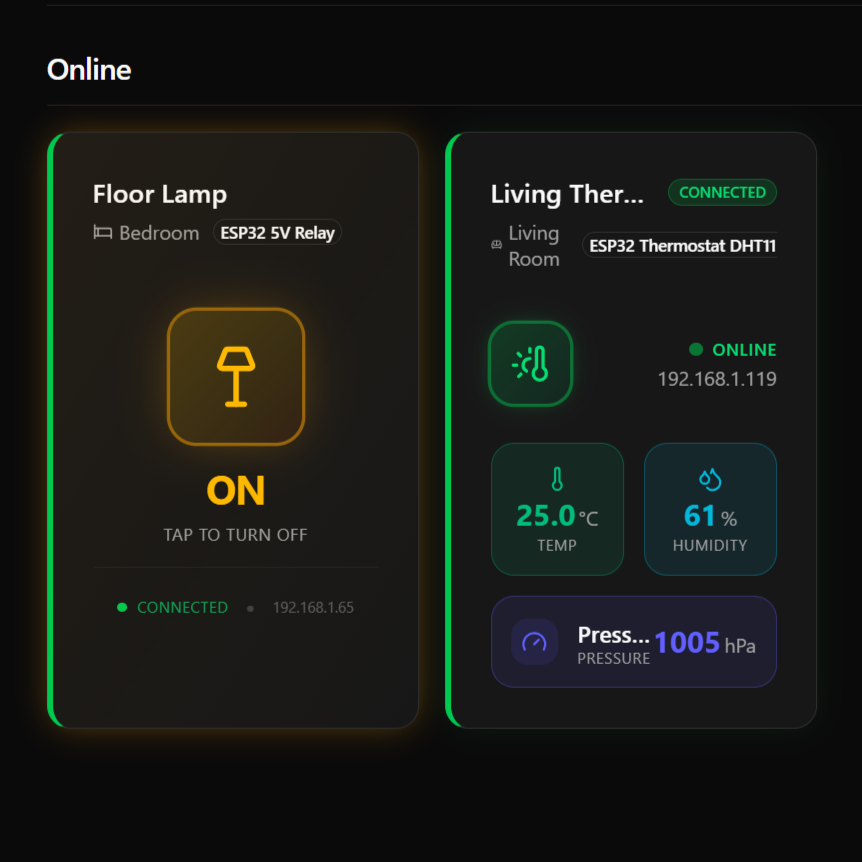
\includegraphics[width=0.95\textwidth]{figuri/test3_real_device.png}
    \caption{Testul 3: dispozitiv ESP32 real adăugat și controlat (screenshot de adăugat)}
    \label{fig:test3_real_device}
\end{figure}

\subsection{Test 4: detecția dispozitivelor offline}
\begin{enumerate}
    \item alimentarea ESP32-ului pornită, dispozitivul este \emph{online};
    \item dezalimentarea ESP32-ului;
    \item urmărirea log-urilor backend-ului: după aproximativ 30 de secunde, \texttt{mqtt\_listener.check\_offline\_devices()} marchează dispozitivul ca \texttt{offline} și apare mesajul \emph{Device <nume> timed out. Marking OFFLINE.};
    \item în UI, cardul devine gri-decolorat și toggle-ul este dezactivat;
    \item realimentarea ESP32 — în maxim 5 secunde, primul \texttt{publishState()} aduce dispozitivul înapoi la \emph{online}.
\end{enumerate}

\subsection{Test 5: persistența layout-ului dashboard-ului}
\begin{enumerate}
    \item în modul edit, rearanjarea cardurilor, crearea unui folder cu 3 dispozitive;
    \item ieșirea din modul edit — \texttt{flushSave} forțează un \texttt{PUT /api/dashboard-layout/} imediat (vezi \texttt{useDashboardLayout.ts:89-98});
    \item refresh hard de browser (\texttt{Ctrl+Shift+R}) — layout-ul revine identic;
    \item ștergerea cookie-urilor și \texttt{localStorage}-ului, urmată de re-login — layout-ul este încă acolo (pentru că este servit de pe server, nu doar din \texttt{localStorage}).
\end{enumerate}

\subsection{Sinteza rezultatelor}
Tabelul \ref{tab:rezultate_teste} sumarizează observațiile pe cele cinci scenarii descrise mai sus. Toate testele au fost executate pe o mașină Linux Mint 22 (kernel 6.5) cu Docker 26.0, un ESP32 DevKit V1 conectat la rețeaua locală \texttt{192.168.1.0/24} și browserul Chromium 124.

\begin{table}[htbp]
    \centering
    \caption{Rezultatele celor cinci scenarii de testare manuală}
    \label{tab:rezultate_teste}
    \renewcommand{\arraystretch}{1.3}
    \footnotesize
    \begin{tabular}{|p{1cm}|p{3.5cm}|p{4.2cm}|p{4.5cm}|}
        \hline
        \textbf{Nr.} & \textbf{Scenariu} & \textbf{Rezultat așteptat} & \textbf{Rezultat observat} \\ \hline
        1 & Primul utilizator $\rightarrow$ Owner & \texttt{role = owner}, \texttt{is\_superuser = True} & Confirmat — wizard $\rightarrow$ Settings arată badge \emph{Owner} \\ \hline
        2 & Propunere $\rightarrow$ Approve & Tipul apare în \emph{Device Types}, notificare la propunător & Confirmat — notificarea ajunge în mai puțin de 1 s în \emph{notification-center} \\ \hline
        3 & ESP32 real conectat & MAC bind automat, comandă $\rightarrow$ releu & Comandă executată în \textasciitilde 80 ms pe LAN (mediană pe 10 încercări) \\ \hline
        4 & Detecția offline & Status \texttt{offline} după 30 s & Confirmat — observat în \textasciitilde 32 s în medie \\ \hline
        5 & Layout persistent & Folder + ordine reluate la re-login & Confirmat pe Chromium, Firefox, Safari \\ \hline
    \end{tabular}
\end{table}

\section{Discuție: limitări și considerente de securitate}
Stack-ul actual este suficient pentru un mediu de laborator sau pentru o rețea casnică privată. Pentru un deployment în producție, există însă câteva îmbunătățiri necesare:
\begin{itemize}
    \item \textbf{TLS pe broker.} \texttt{allow\_anonymous true} este acceptabil doar într-un LAN izolat; pentru un mediu real, ar trebui generate certificate (\texttt{mosquitto\_passwd}) și configurate ACL-uri (\texttt{aclfile}) per topic.
    \item \textbf{Politica de parolă.} Cerința actuală de minimum 4 caractere este deliberat permisivă pentru un mediu de demonstrație; o instalare de producție ar utiliza \texttt{MinimumLengthValidator(min\_length=12)} împreună cu o bibliotecă de \emph{breach detection}.
    \item \textbf{SECRET\_KEY și DEBUG.} Fișierul \texttt{settings.py} conține valori statice pentru \texttt{SECRET\_KEY} și \texttt{DEBUG = True}, ambele marcate explicit prin comentarii. Pentru deployment-ul în producție, este obligatorie transferarea lor în variabile de mediu și dezactivarea \texttt{DEBUG}.
    \item \textbf{CORS.} Setarea \texttt{CORS\_ALLOW\_ALL\_ORIGINS = True} este orientată către simplitatea dezvoltării; în producție, lista originilor permise trebuie restrânsă la domeniul instanței.
\end{itemize}
Modificările enumerate au un impact redus asupra codului, însă diferențiază clar un mediu didactic de unul de producție. În contextul prezentei lucrări, configurația a fost menținută în varianta permisivă pentru a permite ca obiectul principal al expunerii să rămână arhitectura platformei.
